\chapter{Analysis of Twitter's Social Structure}

The social graph of Twitter describes how users are interconnected and fundamentally dictates information flow as Tweets are propagated through its structure. Research so far has focussed on the propagation of information through Twitter's social graph as a result of retweeting. In particular, this research provided an understanding of the patterns produced through retweets and how their properties relate to the users that relay the Tweets. Users with a higher follower count are more likely to have their Tweets retweeted, due to there being more users available to \textit{see} each Tweet, and that some users can have their Tweets forwarded through many hops indeed, so that information may be passed between different communities of users.

In addition to the effects of user influence,  several other factors also influence an individual retweet decision of a given user for a particular Tweet. These include its properties, such as whether, or not, it contains a URL, whether it mentions a particular user, whether the user even has an opportunity to \textit{view} the Tweet, and so on. These factors account for the individual user's retweet decision and the almagamation of every user's retweet decision on the Tweet describes its overall retweetability, which determines how far it can propagate.

However, it is believed that the topology of the network, below the level of user influence and other factors, can play an important role in facilitating (or inhibiting) Tweet propagation by constraining the available retweet pathways between users and communities. Whilst retweet decisions based on Tweet features alone, such as its actual text or the contents of a document a URL it contains refers to, may imply a level of interest in the Tweet, clearly the influence of users can have a very large impact on how many retweets a certain Tweet receives. Thus, abstracting the concepts away from user influence may help in discovering methods for deducing which information is actually interesting.

Twitter's social structure has earlier been described as being built from users creating edges between themselves through the act of \textit{following}. A followship defines the direction of travel of information from the friend to the follower, and this illustrates how users with many followers immediately have their Tweets made available to many more users before any retweeting even takes place. As more edges are constructed between users, the initial audience in terms of the number of users directly receiving the Tweets is increased, and, when the addition of retweets is considered, this effect is amplified. Although other intervening factors have been mentioned in earlier chapters, such as the notion of a user's network awareness and of user influence, the organisation of users on the graph and the differences in observed propagation pattern is a promising route for research towards uncovering the properties surrounding interestingness.

In this chapter, various social network structures are constructed in order to simulate retweet behaviour between users on Twitter. The behaviours are studied with the aim of researching the propagation patterns observed in different network structure types. Non-realistic and realistic graphs are built in order to highlight the low-level propagation characteristics in these networks and the similarities between more realistic simulated networks and Twitter's own social graph. 

This research forms a basis for simulations of Tweets through Twitter's social graph as part of the development of a methodology  for estimating Tweet interestingness from an \textit{expected} level of Tweet popularity. 
 

\section{Propagation Patterns Exhibited by Different Graph Structures}
Although it has been found that Tweets with particular properties may imply a certain quality that affects a user's retweet decision on the Tweet, of interest also is the effect of the  potential presence of a graph `quality', in that particular network structures may have an effect on how Tweets are spread.


In this section, to help in addressing this research area, simulations are carried out in three different network topologies - a path (or `linear') network, a random network, and a scale-free network. In the experiments, individual user \textit{decisions} are used as the bases for demonstrating retweet behaviour.  

The simulation algorithm and ideas behind the model used for generating the simulated users' retweet decisions are adapted from the work carried out in \cite{zhu11} and \cite{peng11}, which introduces methodologies for illustrating Tweet spread through a given network of users, and the simulations can be used to produce a retweet group for a given Tweet. From the analyses of the simulation experiments, of interest is whether, and how, changing the network structure does affect retweet propagation patterns, and whether a simulation can mimic Twitter's own behaviour in terms of retweet spread. If it is the case that the user structure does have a large impact on propagation, and since an individual retweet decision implies that user's interest in a Tweet, then this feature may be used as a basis for estimating interestingness. 

Measuring retweet behaviour is carried out through studying the distribution of retweet group sizes that result from running the experiments, as is described in later sections.

\subsection{Overview of the Simulation Algorithm}
The algorithm covers the simulation of Tweet propagation through a given set of connected users by emulating retweet decisions of each user who receives the Tweet, as is described below. The retweet decision is made using a prediction based on a logistic regression classifier, which is discussed in more detail in Section \ref{section:logistic_regression}.

\cite{zhu11} developed a simulation algorithm which was found to be capable of accurately predicting retweet decisions using a logistic regression. These methods were modified and adapted to fit the purposes of the analyses in this section. The simulation is initialised with a graph of connected users, $G_U$, and a Tweet, $t$, which is introduced to the graph and retweeted between the users as described below. $G_U = (V,E)$ is the social graph of the vertices and edges representing the users who may receive $t$ and the followships between them.

The method begins by initialising a set of users, $S$, to contain the followers of $\aut{t}{O}$. At each time interval, users in $S$ form the set of users to have $t$ or a member of $\rt{t}$ currently on their home timelines and available to retweet. The procedure iterates over timesteps, at each generating a retweet probability on $t$, $P(u,t)$ for each $u \in S$. If $P(u,t)$ is greater than a pseudo randomly-generated $0 \leq r < 1$, then $u$ creates a new retweet of $t$, which is added to $\rt{t}$. $u$ is then removed from $S$ and the followers of $u$ are added to $S$, since these users now also hold $t$ and have the chance to make the retweet decision. $u$ is now unable to retweet $t$ again.

A threshold value, $H$, is used to emulate the notion of the Tweet `decay' experienced when one uses a Twitter client or the web interface. The reasoning behind this is that as time goes by, more and more Tweets arrive onto the recipients' home timelines. This pushes the previous Tweets further down, whether they are interesting or not. Tweets may be ignored and not retweeted if the user has not viewed their home timeline for a while or if the user decides the Tweet is not of a sufficient quality to retweet it. If a Tweet is pushed down to the extent that is out of view, or out of the current page, then the chance of that user retweeting that Tweet is reduced. Thus, if a user is in $S$ for more timestep iterations than specified by $H$, then the user is removed from $S$, meaning that it can no longer have the chance to retweet the Tweet. Users who have retweeted $t$, or are unable to do so (either by having previously retweeted it or by exceeding $H$) are prohibited from being (re-)added to $S$.

The algorithm terminates either when the timesteps thus far iterated exceed the maximum allowed, $T$, or when $S = \left\{\right\}$. This results in the retweet group, $\rg{t}$, which comprises the final members of $\rt{t}$ along with $t$. As in the previous chapter, $\rc{t} = |\rt{t}|$. Therfore, the additional necessary components to run the simulation are a user graph, an initial Tweet, and functionality for generating a retweet probability for each user who receives the Tweet.

Although the described method is mostly the same as the one introduced by \cite{zhu11} and \cite{peng11}, the main differences lie in the selection of and reasoning behind feature selection, as explained over the coming sections.

\newfloat{algorithm}{H}{lop}
\begin{algorithm}
\caption{Simulation of retweet decisions on $t$ in a given graph, $G_U$}
\begin{algorithmic}[1]
\Procedure{simulate}{graph $G_U$, Tweet $t$}
    \State $\rt{t}\gets \left\{\right\}$
    \State $T\gets$ total timesteps
    \State $H\gets$ decay threshold \Comment{Emulate $t$ `slipping down' timeline}
    \State $S\gets \left\{u' \in V(G_U) : \exists \quad \overleftarrow{\aut{t}{O} \quad u'} \in E(G_U)\right\}$
    \State $u.\textrm{TIME\_HELD}\gets 0 \quad \forall u \in V(G_U)$
    \Statex % new line
    \ForAll{$l$ in range $(0,T)$}
        \ForAll{$u \in S$}
            \State $P(u,t)\gets$ retweet probability of $u$ on $t$
            \State $r\gets$ random number in range $[0,1)$
            \If{$P(u,t) > r$}
                \State $r\gets$ new retweet, where $r.\textrm{orig} = t$ \& $\aut{r}{R} = u$
                \State $\rt{t}\gets \rt{t} \cup \left\{r\right\}$
                \State $S\gets S - \left\{u\right\}$
                \State $S\gets S \cup \left\{u' \in V(G_U) : \exists \overleftarrow{u u'} \in E(G_U)\right\}$
            \Else
                \State $u.\textrm{TIME\_HELD}\gets u.\textrm{TIME\_HELD} + 1$
                \If{$u.\textrm{TIME\_HELD} > H$}
                    \State $S\gets S - \left\{u\right\}$ \Comment{$u$ has held $t$ for too long in timeline}
                \EndIf
            \EndIf
        \EndFor
        \If{$|S| = 0$}
            \State Return $\rt{t}$ \Comment{No more users can retweet $t$}
        \EndIf
    \EndFor
    \State Return $\rt{t}$
\EndProcedure
\end{algorithmic}
\label{algo1}
\end{algorithm}


\subsection{Generating a User's Retweet Probability} 
\cite{zhu11} used a predictive model for retweet decisions based on a logistic regression, which was demonstrated to be capable of accurately predicting a user's retweet chance on a given Tweet. The regression was trained on a set of user, Tweet and context features in order to classify a likelihood on the binary decision on each Tweet $t$: retweet or no retweet, such that if $P(u,t) = 1$ then $u$ retweets $t$.


\subsubsection{Machine Learning}
Machine learning is the term given to the family of techniques that allow a program to make predictions for the outcome of unseen instances based on an observed and known history of occurrences. There are many types of machine learning classifiers that are suitable for different purposes, such as for predicting an expected outcome from a set of nominal categories, for predicting a value from a continuous range, or for predicting the \textit{probability} of a binary outcome.

Most machine learning techniques involve the training of a predictive model, which contains the information on known outcomes for a set of features. The model is then used to estimate an unknown outcome, usually with a probability on the \textit{confidence} of the classification, for new sets of instances.

For example, consider three attribute variables, $A$, $B$, and $C$, each of which can be equal to one of two nominal values; \textsc{True} or \textsc{False}. A particular machine learning algorithm trains a model based on its knowledge that;
\begin{itemize}
    \item $A\gets$ \textsc{True}, $B\gets$ \textsc{False} $\Longrightarrow$ $C\gets$ \textsc{True}
    \item $A\gets$ \textsc{False}, $B\gets$ \textsc{False} $\Longrightarrow$ $C\gets$ \textsc{False}
\end{itemize}
Although training of predictive models nearly always involves using more than two instances, the history of these example instances indicate that $C$ is more strongly associated with $A$ than with $B$. As more instances are added showing similar patterns, then the association becomes stronger, to the extent that the classifier will predict $C\gets$ \textsc{True} in instances where $A\gets$ \textsc{True} (and vice versa) with higher confidence.

In this case, $A$, $B$, and $C$ are known as the `features', and a set of such feature values forms the `instance'. Once a trained model has been constructed, the machine learning algorithm will only be able to make predictions using instance features it has knowledge of. For example, if the example classifier was now given an instance containing a feature $D$, then it will not have knowledge of how changes in $D$ will affect $C$'s outcome.

If there is not a strong correlation between the features in a dataset, then the confidence of the classification of a particular feature will be weaker. Although this example has focussed on boolean (nominal) data types, many machine learning classifiers are able to work with features that are higher dimensional nominal values, contunuous reals, and so on, and will apply weights to the different features based on their level of influence over other features in the instance.


\subsubsection{Logistic Regression}
\label{section:logistic_regression}
Much of the research and experiments conducted in this chapter use logistic regression classification techniques in order to classify Tweets and other information. The Background chapter discussed other literature also using logistic regression for social network and retweet analysis \cite{castillo11} \cite{zhu11} \cite{peng11} \cite{naveed11} \cite{hong11}.

The aim of logistic regression analysis is to find the closest model to map correlations between an outcome and a number of input variable features \cite{hosmer13}. Examples of literature already discussed describe the use of logistic regression for `predicting' the probability of a binary outcome in various tests. This type of modelling is appropriate for making predictions on the positive outcome of binary retweet decisions.



\subsection{Summary of Training Features}
\cite{zhu11} used a set of around 50 different features to train the logistic regression for the purposes of simulating retweet decisions, with the retweet outcome (\textsc{True} or \textsc{False}) being the predicted classification in each case. This set included Tweet-related features (such as content analysis, inclusion of URLs, etc.), and network and user features (followships, mentions, etc.).

Since the network structures themselves, and the propagation \textit{patterns}, are what are of interest in this section, the simulation is purposefully and significantly simplified by using far fewer features, yet ones which are features that have been shown to have a stronger influence on the retweet decision. By placing less of the retweet spread responsibility on the individual retweet decisions, and by abstracting them away more from the properties of the social graph, the importance of the structure can become more apparent. The authors of \cite{zhu11} use many features relating to the semantics and content of Tweets, which are also not taken forward here in order to further accentuate the effects of the social structure on dissemination.

As such, each instance comprised the following four features associated with each Tweet, $t$, and where $u$ is the user currently making the retweet decision, \textsc{retweet}. The default value for each feature is \textsc{False};

\begin{table}[h]\footnotesize
\begin{center}
\begin{tabular}{ l | c | l }
	Feature & Data type & Description\\
	\hline
	\hline 
	\textsc{follows}    & \{\textsc{True, False}\} & \textsc{True} if $u \in \fos{\aut{t}{O}}$\\
    \textsc{followed}   & \{\textsc{True, False}\} & \textsc{True} if $u \in \frs{\aut{t}{O}}$\\
    \textsc{mentioned}  & \{\textsc{True, False}\} & \textsc{True} if $u$ is mentioned in $t.\textrm{text}$\\
    \textsc{url}        & \{\textsc{True, False}\} & \textsc{True} if \texttt{http://} or \texttt{https://} in $t.\textrm{text}$\\
    \hline 
    \textsc{retweet}    & \{\textsc{True, False}\} & \textsc{True} if $u \in \rt{t}$\\ 
    \hline
\end{tabular}
\end{center}
\caption{Training features for the logistic regression for simulating retweet decisions}
\label{table:logisticregressionfeatures}
\end{table}

The \textsc{url} feature has, in the literature, often been found as a large impacting feature on retweets in Twitter, especially in \cite{alonso10}, who use it as their basis for determining and identifying interesting Tweets.


\subsection{Training the Model}
In order to train the logistic regression model, data was required from Twitter so that the sets of feature instances could be built. 

Data collection for these experiments again utilised Twitter's REST API, which was queried between March and June 2012 to collect a set of around 18,000 Tweets. The data was collected as part of a random crawl through the social graph, starting at one user and choosing a random follower of the current user to use as the next step. At each stage, information on the current user and on a set of that user's recent Tweets were collected. Tweets that had 0 retweets were collected in order to provide features presenting a negative case when training the regression model and to ensure that there were instances where the \textsc{retweet} feature could be \textsc{False}. In this dataset there are around 2,600 Tweets (15\%) that had been retweeted at least once.

In cases where the collected Tweet had been retweeted, further calls were made to the API to determine the relationships between the authors of the retweets and the original Tweet's author in order to satisfy the required \textsc{follows} and \textsc{followed} features.

Where the collected Tweet had not been retweeted, there are no retweeting users to examine the relationships between. In these cases, further Tweets were retrieved for the user in order to find their retweet rate in terms of the ratio of retweets to Tweets on their user timeline and an analysis of the relationship between these and the original authors. This was used in conjunction with the user's follower and friend count to determine a probability of the `faux' followships. As mentioned, the accuracy of the retweet counts obtained through the simulations is not particularly important; of interest is the propagation patterns observed over the graph structures.

After storage, the regression model was trained using features (see Table \ref{table:logisticregressionfeatures}) extracted from the raw data, with the outcome being the binary retweet decision. The algorithm could then use the model to generate the required retweet probability, $P(u,t)$, by classifying each user's \textsc{retweet} decision outcome at each stage.



\subsection{Running the Simulations}
The logistic regression model, having been trained with the features collected for the training dataset, could then be tested against newly-generated Tweet features in order to output the probability, $P(u,t)$, indicating $u$'s retweet decision likelihood on $t$. The simulation method only produces probabilities for those $u \in V(G_U)$ that actually receive $t$ and have a chance to retweet it. Since some of the features used rely on the relationships of the current $u$ to $\aut{t}{O}$, not every user in the graph will have the same value for $P(u,t)$.

For each simulation experiment, a network of users was generated according to a structured model, as described in the next section. A Tweet object was then constructed and contained information on whether or not it contained a URL and if it mentioned one of the users in the generated network. 

In each network analysis, the same set of Tweets was used. This set comprised Tweets generated from many feature combinations. Various parameters - such as $H$, the size of the user network, $G_U$ to be generated, and any weightings on the decision probability prediction generator - were altered in the simulations in order to affect the visibility of any correlations in the propagation patterns produced by the different structure types. As such, the \textit{volume} of retweet counts produced are not comparable across the structure analyses, but the correlation patterns are.


\subsection{Network Analyses}
In this section, three network structures are assessed in terms of the differences in the patterns of propagation each permits. Each generated graph is \textit{directed} in order to illustrate the followships between the user nodes, and to support the use of the \textsc{follows} and \textsc{followed} features required in the decision probability calculation.


\subsubsection{Path Network}
The first assessment involved illustrating the propagation pattern observed in the most basic social network structure; a path network. Albeit non-realistic in practice, these graphs represent the fundamental structure of a connected `world' of users.

A linear directional path network consists of the graph of users, $G_U$, of size $n$;
\[
    n = |V(G_U)| = |E(G_U)| + 1
\]
where; 
\[
    \exists \quad \overleftarrow{u_i \quad  u_{i+1}} \in E(G_U) \quad \forall \quad 1 \leq i < n
\]
As a result, each $u \in V(G_U)$ has precisely one follower and one friend, except the users $u_n$ and $u_1$ respectively. $n$ is the only parameter necessary in the construction of this user graph.

\begin{figure}[h]
\centering
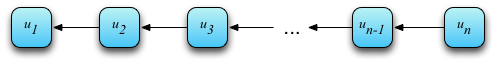
\includegraphics[scale=0.8]{4.Chapter2/Media/path_network.png} 
\caption{Example of a path network.}
\label{fig:path_network}
\end{figure}

In this graph, the size of the retweet group is, by definition, equal to the depth of penetration, as there is only one path (or retweet chain) available for propagation to occur along. As such, in each case, the retweet tree representing a resultant retweet group formed in this type of network will have the same structure as the graph itself, with a size dependent on the collective retweet decisions of the users.

Since each internal user has only one follower, the likelihood of each progressive user in the graph being able to view the Tweet in order to make the retweet decision reduces, and thus the retweet count is much more likely to tail off sooner than in graphs with more propagation avenues. This is also due to the fact that each retweet can only reach an audience of size 1 at each time step, and thus the `survival' of the Tweet cannot rely on a summation of many users' retweet decisions. The actual retweet \textit{decision} is not affected by a user's position in terms of `distance' from the source except through the effect of the regression features.

\begin{figure}[h]
\centering
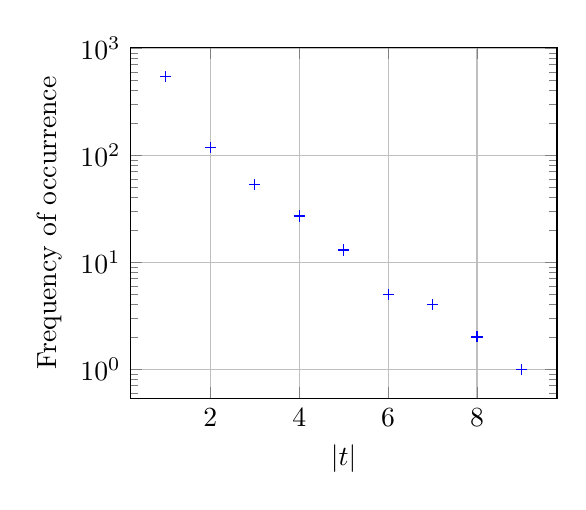
\begin{tikzpicture}
 \begin{semilogyaxis}[
        xlabel=$|\rg{t}|$,
        ylabel=Frequency of occurrence,
        width=7cm,
        grid = major]
    \addplot[only marks,mark=+,blue] plot coordinates {
        (1,540)  (2,118)  (3,53) (4,27) (5,13) (6,5) (7,4) (8,2) (9,1) (10,0)
    };
\end{semilogyaxis}
\end{tikzpicture}
\caption{Frequency distribution of retweet group sizes in path network simulations}
\label{fig:linear}
\end{figure}

The likelihood of a particular user achieving the opportunity to receive the Tweet, in order to then retweet it, becomes the product of the probability function the further it travels through the graph, in which user $u_i$ requires each user from $u_1$ to $u_{i-1}$ to first receive it and then make a positive retweet decision. For example, if each user has probability $p$ of retweeting the Tweet, then each user's chance of receiving the Tweet is $p^{i-1}$, where $i$ is the position of the user in the graph. A user can only make a retweet decision on $t$ once it has been received.

The path network analyses involved 50 repeat simulations of the set of Tweets on a graph of size $n = 1000$. A timeline threshold ($H$) of 30 was used to represent the maximum time a Tweet is permitted on a user's timeline before it is no longer retweetable, for reasons discussed earlier. 

As might be expected, the frequency distribution of retweet group sizes in Figure \ref{fig:linear} shows a half-life type behaviour demonstrating the logarithmic pattern with many small retweet groups followed by a series of exponentially smaller groups. This user structure illustrates well how some users that might find the Tweet interesting, and who may then decide to retweet it, do not even get the chance to view it in order to \textit{make} that decision. Although this is accentuated in this structure, the same principle applies to any non-complete social graph, and demonstrates how the way in which users are connected can have a large impact on the overall retweetability of a particular Tweet.


\subsubsection{Random Network}

\begin{figure}[h]
\centering
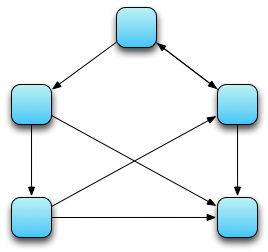
\includegraphics[scale=0.8]{4.Chapter2/Media/random_network.png} 
\caption{Example of a random network where $n = 5$ and $P_c = 0.5$.}
\label{fig:path_network}
\end{figure}

The random network was the next user structure to be analysed. Although it is certainly more similar to a real-life social graph than a path network, it is much more basic and uniform and does not consider user communities and clusters or different levels of influence in users in terms of differences in follower and friend counts.

A random social network is in this case based on the Erd\H{o}s-R\'{e}nyi model \cite{erdos60} and defined as a graph, $G_U$, where $n = |V(G_U)|$, consists of each user, $u \in V(G_U)$, having the connection probability $P_c$ of following each other $u_i \in V(G_U) \forall 0 \leq i \leq n$ and where $u_i \neq u$. Thus, as $P_c$ is increased, then so does the likelihood of $u$ following a $u_i$, causing the network to have a greater overall edge density. In general, therefore, the average number of followers and friends of a user is proportional to $P_c.n$. The only parameters needed for constructing such a graph are $n$ and $P_c$.

\begin{figure}[h]
\centering
\begin{tikzpicture}
 \begin{semilogyaxis}[
        xlabel=$|\rg{t}|$,
        ylabel=Frequency of occurrence,
        width=7cm,
        grid = major]
    \addplot[only marks,mark=+,blue]
       file {4.Chapter2/data/random.dat};    
\end{semilogyaxis}
\end{tikzpicture}
\caption{Frequency distribution of retweet group sizes in random network simulations}
\label{fig:random}
\end{figure}

As with the path network analysis, a graph size of $n = 1000$ was used under 50 simulations with the value of $H = 30$. The distribution in Figure \ref{fig:random} was generated using a value of $P_c = 0.01$, meaning that, on average, each user had 10 followers and 10 friends and was felt to be representative given the size of the entire graph.

The frequency distribution in Figure \ref{fig:random} demonstrates a very large proportion of mid-range values for $|\rg{t}|$, indicating that Tweets tend to have a consistent spread amongst the network, as might be expected. There are few smaller groups since there are no users that have disproportionately smaller spheres of influence, and each user has many incoming edges and a similar number of outgoing edges. This explains the smaller number of lower-range retweet group sizes observed in the distribution. However, as in any distribution so far examined, the number of larger retweet groups must eventually tail off due to the natural eventual reduction in positive retweet decisions being successively made as propagation chains increase in length.


\subsubsection{Scale-Free Network}
The final network structure examined in this section is the scale-free network. Also known as `small world', scale-free graphs are generally known to be representative of the general structure of `real-life' and online social networks \cite{mislove07} and, indeed, they are also used to describe the interconnections of real-world properties, such as friendship groups and food webs \cite{guido07} \cite{hein06}. Essentially, scale-free networks dictate that there are a small number of nodes with a high degree and many nodes with a low degree, and are usually generated through some form of preferential attachment algorithm. Thus, this type of network has support for the consideration of user communities and influential users in terms of those demonstrating a disproportionately large follower count. The other user structures studied do not have the scope for emulating this property of inconsistent interconnection between the user nodes.

Scale-free networks are constructed such that the distribution of the degree of the graph's nodes follow a power-law in that the distribution of the number of vertex edges across the graph is logarithmic. For these analyses, NetworkX\footnote{http://networkx.lanl.gov}, a Python graph and networking package, was used to generate directed scale-free graphs of users, based on a graph size, $n$, and other arguments, including $\delta$-out, as the graph construction parameters. 

For the scale-free analysis, the same graph construction and simulation parameters were used as in the previous analyses. $\delta$-out represents the bias for a node's selection for out-degree from the other available nodes, and was set to a value of 0.7 to improve the clarity of the distribution result.

\begin{figure}[h]
\centering
\begin{tikzpicture}
 \begin{loglogaxis}[
        xlabel=$|\rg{t}|$,
        ylabel=Frequency of occurrence,
        grid = major,
         legend style={at={(0.5,-0.27)},anchor=north,legend cell align=left},
        legend entries={Twitter data, Generated scale-free data}]
    \addplot[only marks,mark=+,red]
       file {4.Chapter2/data/comparison-real.dat};
    \addplot[only marks,mark=+,blue]
       file {4.Chapter2/data/comparison-scale-free.dat};
\end{loglogaxis}
\end{tikzpicture}
\caption{Comparison of retweet group size distributions from scale-free graph simulations and data from Twitter's own social graph}
\label{fig:real-scalefree}
\end{figure}

From simulations of the algorithm through these scale-free networks, a logarithmic trend is observed similar to that demonstrated from the `real' Twitter data analysed in the previous chapter and published in \cite{webberley11}, and the similarities in the distribution pattern is illustrated by Figure \ref{fig:real-scalefree}.


\subsection{General Comparison of Propagation Characteristics across Different Graph Structures}
In this section, three different network structures have been compared, and whilst the path network is very unrealistic as a representation of a social network, the differences in propagation behaviour presented by each do show how the interconnection of users on the graph can have a large effect on the spread of a Tweet. A small set of features to govern retweet features were used in order to accentuate the difference made by the user structures themseleves.

This has demonstrated that, in addition to the processes behind a user's individual retweet decision, the eventual spread of a Tweet also depends on how the original author's local network is arranged. Thus, the retweet decision of each involved user along with the available information pathways provided by the underlying social structure both contribute to the overall retweetability of a Tweet. 

If there are many edges in the network, such as in the case of the random network, then there are many more routes for peopagation to occur down to and from each user, due to the relatively large in- and out-degree of each user node on the graph. This increases the number of users who end up receiving the Tweet and then have the chance to make a retweet decision. This resulted in there being a larger distribution of larger retweet group sizes than smaller ones, before naturally diminishing again. 

\begin{figure}[h]
\centering
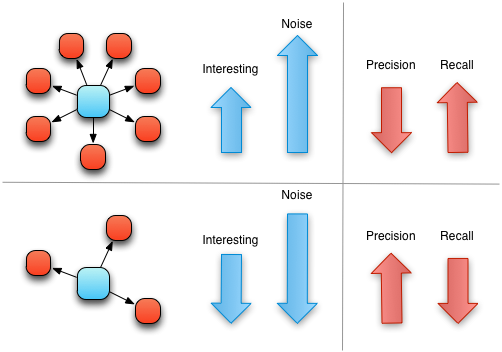
\includegraphics[scale=0.8]{4.Chapter2/Media/precision_recall.png} 
\caption{Comparing the effects of followship decisions on precision \& recall.}
\label{fig:precision_recall}
\end{figure}

Despite this high throughput of retweets, which provides a high level of information \textit{recall} for the users, the random graph structure is likely to demonstrate a low \textit{precision} in terms of the interestingness of the received Tweets. This is due to the large number of users having the opportunity to retweet the Tweet, increasing the chance that `noisy' information will be filtered through. As illustrated in Figure \ref{fig:precision_recall}, it is generally the case that if a person follows more users, they will receive exponentially more noise due to its prevalence over the interesting information (a decrease in precision), yet will likely receive more of the interesting information that is available (an increase in recall).

The path network demonstrated the opposite effect in that its nodes can only follow a maximum of one other node. This demonstrated very poor propagation, and required its simulation parameters to be altered to facilitate retweet behaviour more significantly than in the other graph structure analyses in order to produce any observable pattern. The results showed that propagation down a single allowed chain cannot be an effective way to spread Tweets, as it required each user in the chain to retweet it so that the successive users can have a chance to view it.

Similarly, in Twitter, users who follow very few others are likely to be more selective about who they follow. They will therefore achieve a greater precision in terms of the interestingness of information received, but the recall will be much smaller (Figure \ref{fig:precision_recall}). Generally, it is impossible to achieve a perfect precision and recall as it is likely that there will always be interesting information not being received, and any noise that is received at all will reduce the precision.

Whilst the scale-free network does not have the same general propagation throughput as the random network, it does demonstrate retweet patterns similar to those observed in data from Twitter's own social graph. This complements the findings of \cite{mislove07} and \cite{hein06} in terms of online social networks emulating real-life social networks having scale-free properties. This type of structure supports areas of the graph with denser communities, as is shown to exist by \cite{java07}, and have the potential for facilitating very large numbers of retweets if influential users are involved, but illustrate how Tweets `travelling' through less dense areas (and less-influential users) will not be as demonstrably popular.



\section{Using the Social Graph as a Method for Inferring Interestingness}
The graph analyses in the previous section have demonstrated a method for generating a $\rg{t}$ for a given Tweet, $t$. Since $\rc{t} = |\rg{t}| - 1$, then the same simulation algorithm can be used to estimate a retweet count for a given Tweet. The analyses conducted in the previous section relied on modelling the retweet \textit{decisions} made by the users, which individually account for that particular user's interest in that Tweet. Although it has been previously discussed that the overall retweet count cannot realistically be used alone for determining the level of interest in a Tweet, it is clear that interestingness of a Tweet is certainly based on a \textit{function} of the culmination of positive retweet decisions being made on the Tweet.

This notion is based on the idea that if a Tweet is more popular than the model predicts, then there is something about that Tweet that makes it more \textit{interesting} than similar Tweets that are less popular, such as a piece of breaking news or a link to a controversial article. For example, consider the case of two Tweets, written by the same author, and both containing the same instances of feature values in that they both contain a URL and mentions a user. If one of these Tweets achieves significantly more retweets than the other, then there must be some non-structural feature of the more popular Tweet that makes it stand out to the audience, and thus allows it to be perceived as more \textit{interesting}. This is because the features taken into account are static, and do not address any semantics of the actual content of the Tweet.

Similarly, if most Tweets of a user achieve between one and two retweets, then the expected retweet count for this user's future Tweets is likely to be similar. If, however, the author posts a Tweet which achieves an observed total of 10 retweets, then this is more popular than expected. If a Tweet achieves one or zero retweets, then this is as expected or less than expected, and is therefore not interesting.

\begin{myproposition}
\label{proposition:1}
The interestingness of a Tweet is a function of its expected and observed popularity. In particular, that a Tweet should be labelled as interesting if it is more popular than it was expected to be.
\end{myproposition}

This form of analysis is akin to anomaly detection and, in particular, the Helmholtz principle, which is defined by \cite{balinsky11} to be the deviation of interesting events from the randomness of the non-interesting events surrounding them. In the context of Proposition \ref{proposition:1}, exceptionally popular (or unpopular) Tweets can be represented by the interesting events, and the \textit{norm} of expected Tweet popularity is analogous to the randomness of non-interesting events.

Figure \ref{fig:helmholtz} helps demonstrate this behaviour in the context of Proposition \ref{proposition:1}, in which there is a `baseline' of expected Tweet popularity given by the properties of the Tweet and its environment. The exceptional, or anomalous Tweets, are the ones that are significantly different from the baseline; those that are much higher than this baseline are labelled as interesting since they are more popular than their features imply, and vice-versa.

\begin{figure}[h]
\centering
\begin{tikzpicture}
\begin{axis}[
        ylabel=Tweet popularity,
		xlabel=Feature amalgamation,
		ymax=200,
		xmax=20,
		xmin=0,
        yticklabels={,,},
        xticklabels={,,}
        ]
    \addplot[only marks,mark=+,blue] coordinates{
        (0,3)(1,6)(2,8)(3,17)(4,21)(5,27)(6,29)(7,35)(8,39)(9,48)(10,52)(11,53)(12,59)(13,61)(14,67)(15,71)(16,73)(17,81)(18,85)(19,92)(20,100)
    };
    \addplot[only marks,mark=+,blue] coordinates{
        (3,37)(5,59)(10,11)(14,130)(18,23)
    };  
\end{axis}
\end{tikzpicture}
\caption{Conceptual example illustration of Tweet popularity as a function of their properties}
\label{fig:helmholtz}
\end{figure}

As such, a method is proposed based on the following two criteria;
\begin{itemize}
    \item $\rc{t} > \ec{t} \Longrightarrow t$ is interesting
    \item $\rc{t} \leq \ec{t} \Longrightarrow t$ is non-interesting
\end{itemize}
where $\ec{t}$ is the expected retweet count of $t$.

Although it was found in the previous chapter and in other relevant literature that pseudo-generated scale-free networks can be representative of Twitter's own social structure, a user's actual own local social network would more accurately portray the links between the users surrounding the original author of a Tweet. By constructing a network based on a user's own local network, then the method would effectively be simulating the Tweets' propagation through the edges representing the followships of the real and appropriate users in Twitter's social graph.

Thus, in the simulations, the user in question is $\aut{t}{O}$, $t$ is the Tweet to be simulated and initially $S = \fos{\aut{t}{O}}$. At each timestep, each user in $S$ would have the opportunity to retweet $t$, and therefore, by running the simulation multiple times, an estimation of $\ec{t}$ can be obtained.\\
In particular, the method follows these steps;
\begin{enumerate}
    \item Select a user, $u$, from Twitter to be $\aut{t}{O}$
    \item Collect $u$'s local follower network 
    \item Collect a set of $u$'s recent Tweets
    \item Construct a network based on the users and edges of the collected network
    \item Simulate the collected Tweets through the constructed network using the simulation algorithm.
\end{enumerate}

This procedure would provide an estimated retweet group size for each Tweet, which could then be compared to the actual observed retweet count of the Tweet on Twitter to help towards deducing the interestingness.


\subsection{Data Collection}
In order to simulate Tweets through Twitter's own social graph, data on its users and edges is required so that a copy of the graph can be built locally. This is necessary for the users' retweet decisions to be modelled and to keep track of which users are able to receive the Tweets.

Ideally, the actual social graph would be used, but due to the scaling properties encountered in a breadth-first traversal of Twitter's social graph, it became infeasible to collect a user's local network containing users more than two edge `hops' away from the source user under the rate limitations of Twitter's REST API. As previously described, v1 allowed 350 calls to the API each hour for each authenticated Twitter account. One call, for example, was required to obtain a list of up to 5,000 user IDs representing the followers of a particular user - the users one hop from the source user. An additional call would then be required to collect each of these user's own followers in order to provide the 2-hop representation of the local network from the source user.

For a user with a follower count of 700, a total of 701 API calls would be required to collect the user's local network within two hops - the one to retrieve the source user's immediate followers, and then one further call for each of the 700 followers. This would take over two hours of collection, and to collect the third hop would require another exponential number of API calls. If each of the 700 followers of the source user has, on average, 200 followers, then this would require  a further $700 \times 200 = 140,000$ API calls, which, in total, equates to over 402 hours of data collection time. Although some follower overlap is likely to be present among the users two hops away, when one considers that this is simply the time taken to collect the local network for \textit{one} user, then it becomes clear that this must still be an impractical approach.

Observation \ref{observation:path-length} states that the vast majority of retweets do actually occur \textit{within} two hops of the source user, in that the most significant number of retweet groups analysed had a maximum path-length of less than three. In addition, as mentioned, online social networks are `closer' than real-life social networks, and was found to have a value of around four degrees of separation in Facebook. These points help to justify the decision made to classify a user's local network as those users and edges existing within two hops from the source user.

In June 2012, the Twitter REST API was used in order to conduct a random walk through Twitter's social graph. Starting by selecting an initial user, an edge expressing the followship of a random follower was chosen in order to select the next user. This continued for each of the selected users in turn and, for each user selected, the most recent 300 Tweets and surrounding information was collected along with that user's local follower network within two hops. The friend network (i.e. the outward edges from each user) was ignored, as only the directional outward flow of information from the source user was useful in this experiment. If, at any stage, the currently selected user did not have any followers, the collection algorithm backtraced to the previous user and another follower was selected instead. The crawler continued until the rate limit for the current request window was met, at which time the current data state was stored, and then waited until the rate-limit was reset before continuing.

The data collection resulted in a set of 33 Twitter users, each with a full 2-hop local network collected and a set of up to 300 Tweets. In total, around 10,000 Tweets were stored as a result of the crawl to be used in the simulations. It was decided that the previously trained regression model would be re-used as part of the retweet decision engine in this experiment also, and so no further training data was required to be collected. From the Tweets collected, the \textsc{url} and \textsc{mentioned} features could easily be indentified, and the two user features could be extracted under the same process as the one used in the network simulations in the previous section.

For each Tweet collected, a simulation could now be run in order to provide an expected retweet count for that particular Tweet. By comparing this value to the actual retweet count expressed by the Tweet, which is returned as part of the standard Twitter API call, an indication of whether or not the Tweet is interesting could be obtained.



\subsection{Validating the Accuracy of Inference Results}
In order to test the validity of the results, it was necessary to use human asessment on each of the evaluated Tweets to check for agreement between the interestingness inferences made by the algorithm and by humans. Although interestingness is a subjective notion, the validations were carried out in such a way to emphasise a \textit{global} level of interest in terms of the general separation between noisy and un-noisy Tweets.


\subsubsection{Crowdsourcing Validations}
Crowdsourcing is a technique that has grown in popularity over many domains in recent years, including in the media, reviews services, sensor networks, and others. Essentially, crowdsourcing involves the use of many people (or, in some cases, devices) providing input or results on a given task. Services such as Google Maps\footnote{http://maps.google.com}, TripAdvisor\footnote{http://tripadvisor.co.uk}, and Stack Overflow\footnote{http://stackoverflow.com} respectively use crowdsourcing for obtaining information (such as photos) on geographic locations, service reviews, and programming assistance. Its use means that the crowdsourcers can easily receive lots of input with very little additional work, since the load is spread amongst many people.

Crowdsourcing has also proved to be a useful asset in research as it facilitates the harvesting of many inputs, from diverse opinions and views, much more quickly than without it, and it is a useful tool for validating data. Many crowdsourcing services are active on the Internet to cater for different use-cases.

Amazon's Mechanical Turk\footnote{http://mturk.com} allows crowdsourcers to create small jobs (known as `microtasks') to be completed by crowdsourcees, known as Mechanical Turk Workers (MTWs), who have an account on the website. The crowdsourcer describes the particular microtask in terms of what is expected of the MTWs and also determines the amount paid for the task. A single microtask completed by a particular MTW is known as a `judgment', and MTWs are paid for each judgment he/she completes. The crowdsourcer can define certain criteria on the microtasks, such as allowing each MTW to only complete one microtask.

Due, at this time, to Mechanical Turk's availability to only US credit card holders, a third-party service, CrowdFlower\footnote{http://crowdflower.com}, was used instead to submit the microtasks to Amazon's system in order to be completed by the workers. 


\subsubsection{Aims of the Validations}
The purpose of the use of crowdsourcing was for evaluating the effectiveness of the interestingness inferences made through the comparison between an expected and observed popularity of a given Tweet. Of particular concern was the correlation between those Tweets that the algorithm denoted as interesting and the Tweets that humans found interesting.

Since the accuracy of the various components of the technique could not be known until they were properly validated, it was decided that the crowdsourcing would initially be run as a pilot test in order to identify the presence of any correlations. If this was sufficiently successful, then a further and more rigorous test would take place, involving more workers.


\subsubsection{Constructing the Questions}
The microtasks presented to the MTWs each consisted of a question containing five Tweets that were selected at random from the experimental set. Each question asked the MTWs to select which one of the five Tweets was the most interesting and which one was the least interesting. The validations were set up so that each of the questions was assessed by at least three different MTWs.

\begin{figure}[h]
\centering
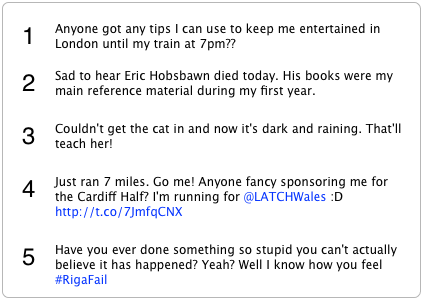
\includegraphics[scale=0.8]{4.Chapter2/Media/mtk_question.png} 
\caption{Example question for the MTWs: "Select the most interesting Tweet and the least interesting Tweet from the five shown"}
\label{fig:mtk_question}
\end{figure}

Figure \ref{fig:mtk_question} shows an example of a question asked of the workers. It demonstrates also how the MTWs were not provided with any additional context, such as the author's username or the post date and time, for any of the Tweets to be evaluated.

Although Tweet selection was random, those whose content starts with a user's ``@'' username (i.e. `@-replies') were excluded, since these Tweets typically form part of a conversation between a small number of users and are unlikely to convey any interest to those not directly involved. The final validation set consisted of a total of around 4,300 Tweets to be assessed in the questions, and MTWs were encouraged to follow links to any websites or media included in the Tweets' contents as part of their evaluations. For each question ansewered, MTWs were paid \$0.05. 


\subsubsection{Inference Performance Validation Results}
\label{section:initial_inference_results}
The Mechanical Turk validation took place between the 7th and 11th December 2012. Table \ref{table:mtk_data_1} provides further information about the validation tests. An assessment is defined as a MTW answering a particular question with his/her opinion on the most interesting and least interesting Tweet. Since there were 856 questions, there were 2568 assessments in total.

\begin{table}[h]\footnotesize
\begin{center}
\begin{tabular}{ l || r }
     Information key & Value\\
     \hline
     \hline
	 Total assessments by MTWs & 2568\\
	 Number of distinct questions & 856\\
	 Number of unique MTWs & 177\\
	 Number of unique Tweets & 4280\\
	 \hline
	 Num. questions with $\geq \frac{2}{3}$ agreement on most interesting & 510\\
	 Num. questions with $\geq \frac{2}{3}$ agreement on least interesting & 493\\
	 \hline
	 Amount paid to MTWs per assessment & \$0.03\\
	 Total amount paid & \$77.04\\
     \hline
\end{tabular}
\end{center}
\caption{Information on the Mechanical Turk validation results.}
\label{table:mtk_data_1}
\end{table}

A confident answer is defined as the case in which at least two of the three MTWs answering a particular question agree on the most interesting and least interesting of the Tweets. It is assumed that if at least two people agree on a piece of content being interesting, then this provides further strength to the individual assessments, and any questions that were not confident were excluded from the following validation analysis.

Through the retweet simulations and algorithm for each Tweet, an 86\% accuracy was achieved in terms of correctly predicting the actual retweet count - the cases where the expected retweet count is equal to the observed retweet count. In around 30\% of cases, a Tweet that was determined to be interesting through the methodologies described in this chapter was also verified as interesting by the agreeing MTWs.

This is a relatively low accuracy, and while it does mean that the method was able to correctly identify an interesting Tweet from a set of five in 30\% of cases and the random performance of selecting an interesting Tweet could not reach this accuracy, it is not a strong enough result to describe the method as being suitable in the general inference of interesting Tweets. 

As such, further investigation would be required to address the method with the aim of improving this performance.


\subsection{Improving The Interestingness Inference Performance}
Proposition \ref{proposition:1} is still considered to be a viable way of addressing the problem of identifying interesting information for the reasons discussed earlier. However, a more convenient and accurate method is clearly required for acquiring the \textit{expected} retweet value.

The issue with the current method is two-fold; a large volume of data is required in order to reconstruct the Tweets' authors' local networks in which to simulate the Tweets, which leads to the second problem of only being able to simulate Tweets from authors in sparser local networks. Under the current scheme, only users with a small enough local network (i.e. users that have lower folower counts) can realistically be evaluated, due to the collection criteria discussed previously, meaning that the methodology cannot be used in the general case. Although a high accuracy was achieved in predicting the \textit{correct} retweet counts for the Tweets assessed in this section, most of these Tweets only actually had an observed retweet count of 0 or 1. This is the by-product of the previous issue in that only users with fewer followers could have their Tweets simulated, and these users will therefore typically receive few retweets per Tweet. Ideally, the methodology should have the capabilities to be applied to any type of user and any Tweet on Twitter.

Additionally, this method alone does not make efforts towards evaluating the \textit{level} of Tweet interestingness. Instead of the binary interesting / non-interesting decision, it would be more useful to award each Tweet a score denoting the estimated interestingness of the Tweet. The further importance and usefulness of this is explained in further detail in the following chapter.


\section{Chapter Summary}
In this chapter, an analysis of propagation through differing structures of user connections on social graphs has been conducted. From this, a potential methodology for inferring interestingness of Tweets has emerged, which, despite being negatively impacted by various factors in its current form, shows promise as a suitable technique towards assisting in this task.


\subsection{Network Structure Analysis}
A logistic regression model was built as part of a simulation algorithm in order to anaylse the propagation characteristics of three different network structures; a path network, a random network, and a scale-free network. 

Although the actual retweet counts of simulated Tweets in each network structure are not comparable due to the parameter alterations that were required in order to amplify visible results, the actual \textit{pattern} of propagation in terms of the distribution of retweet group sizes was found to be different in each structure and for differing reasons. In addition, the scale-free network was found to express a similar pattern to that observed from the data on retweet group sizes discussed in the previous chapter.


\subsection{Interestingness Inference Methodology}
The model and techniques behind the network structure analyses were then applied to the goal of detecting the interestingness of Tweets based on the comparison of the expected retweet value, generated through the same algorithm used to simulate Tweets in the network analyses, and the actual observed retweet count of the Tweet.

Validating the methodology showed that the technique is not particularly useful in determining interesting information, and its other drawbacks, such as its application only realistically being available to Tweets from non-influential users, mean that the technique cannot be used in the general case. Further to this, the data collection required is not suitable for quick evaluations and may not remain accurate over time even after collection due to the continuous changing nature of the edges in online social networks as users create and destroy followships. This is particularly impactful in this case as there are many users involved even in a user's 2-hop local network.

In the next chapter, the methodology for generating expected retweet counts is adapted with the aim of improving its validation performance, the ease of preparation through data collection, and of addressing the methodology's current restrictions on the types of users it is suitable for. It is known from work in this chapter that the network structure plays an important role in information propagation, so this and more environmental features are taken forward as part of the improvements. 
